\section{Vandermonde matrix}

The code of any shared modules for question 2 is given by:
\lstinputlisting[firstnumber=1, firstline=1, lastline=120]{2_vandermonde_matrix.py}

\subsection{a}

TODO(For all routines you write,explainhow they work in the comments of your code andargueyourchoices)
TODO(This includes discussing your plots in their caption)
TODO(Per main question, the code of any shared modules. Per sub-question, an explanation of what you did. Per sub-question, the code specific to it. Per sub-question, the output(s) along with discussion/captions)
TODO(Add plotting code.)


\lstinputlisting[firstnumber=125, firstline=125, lastline=146]{2_vandermonde_matrix.py}

\lstinputlisting{vandermonde_matrix.txt}

\begin{figure}[h!]
    \centering
    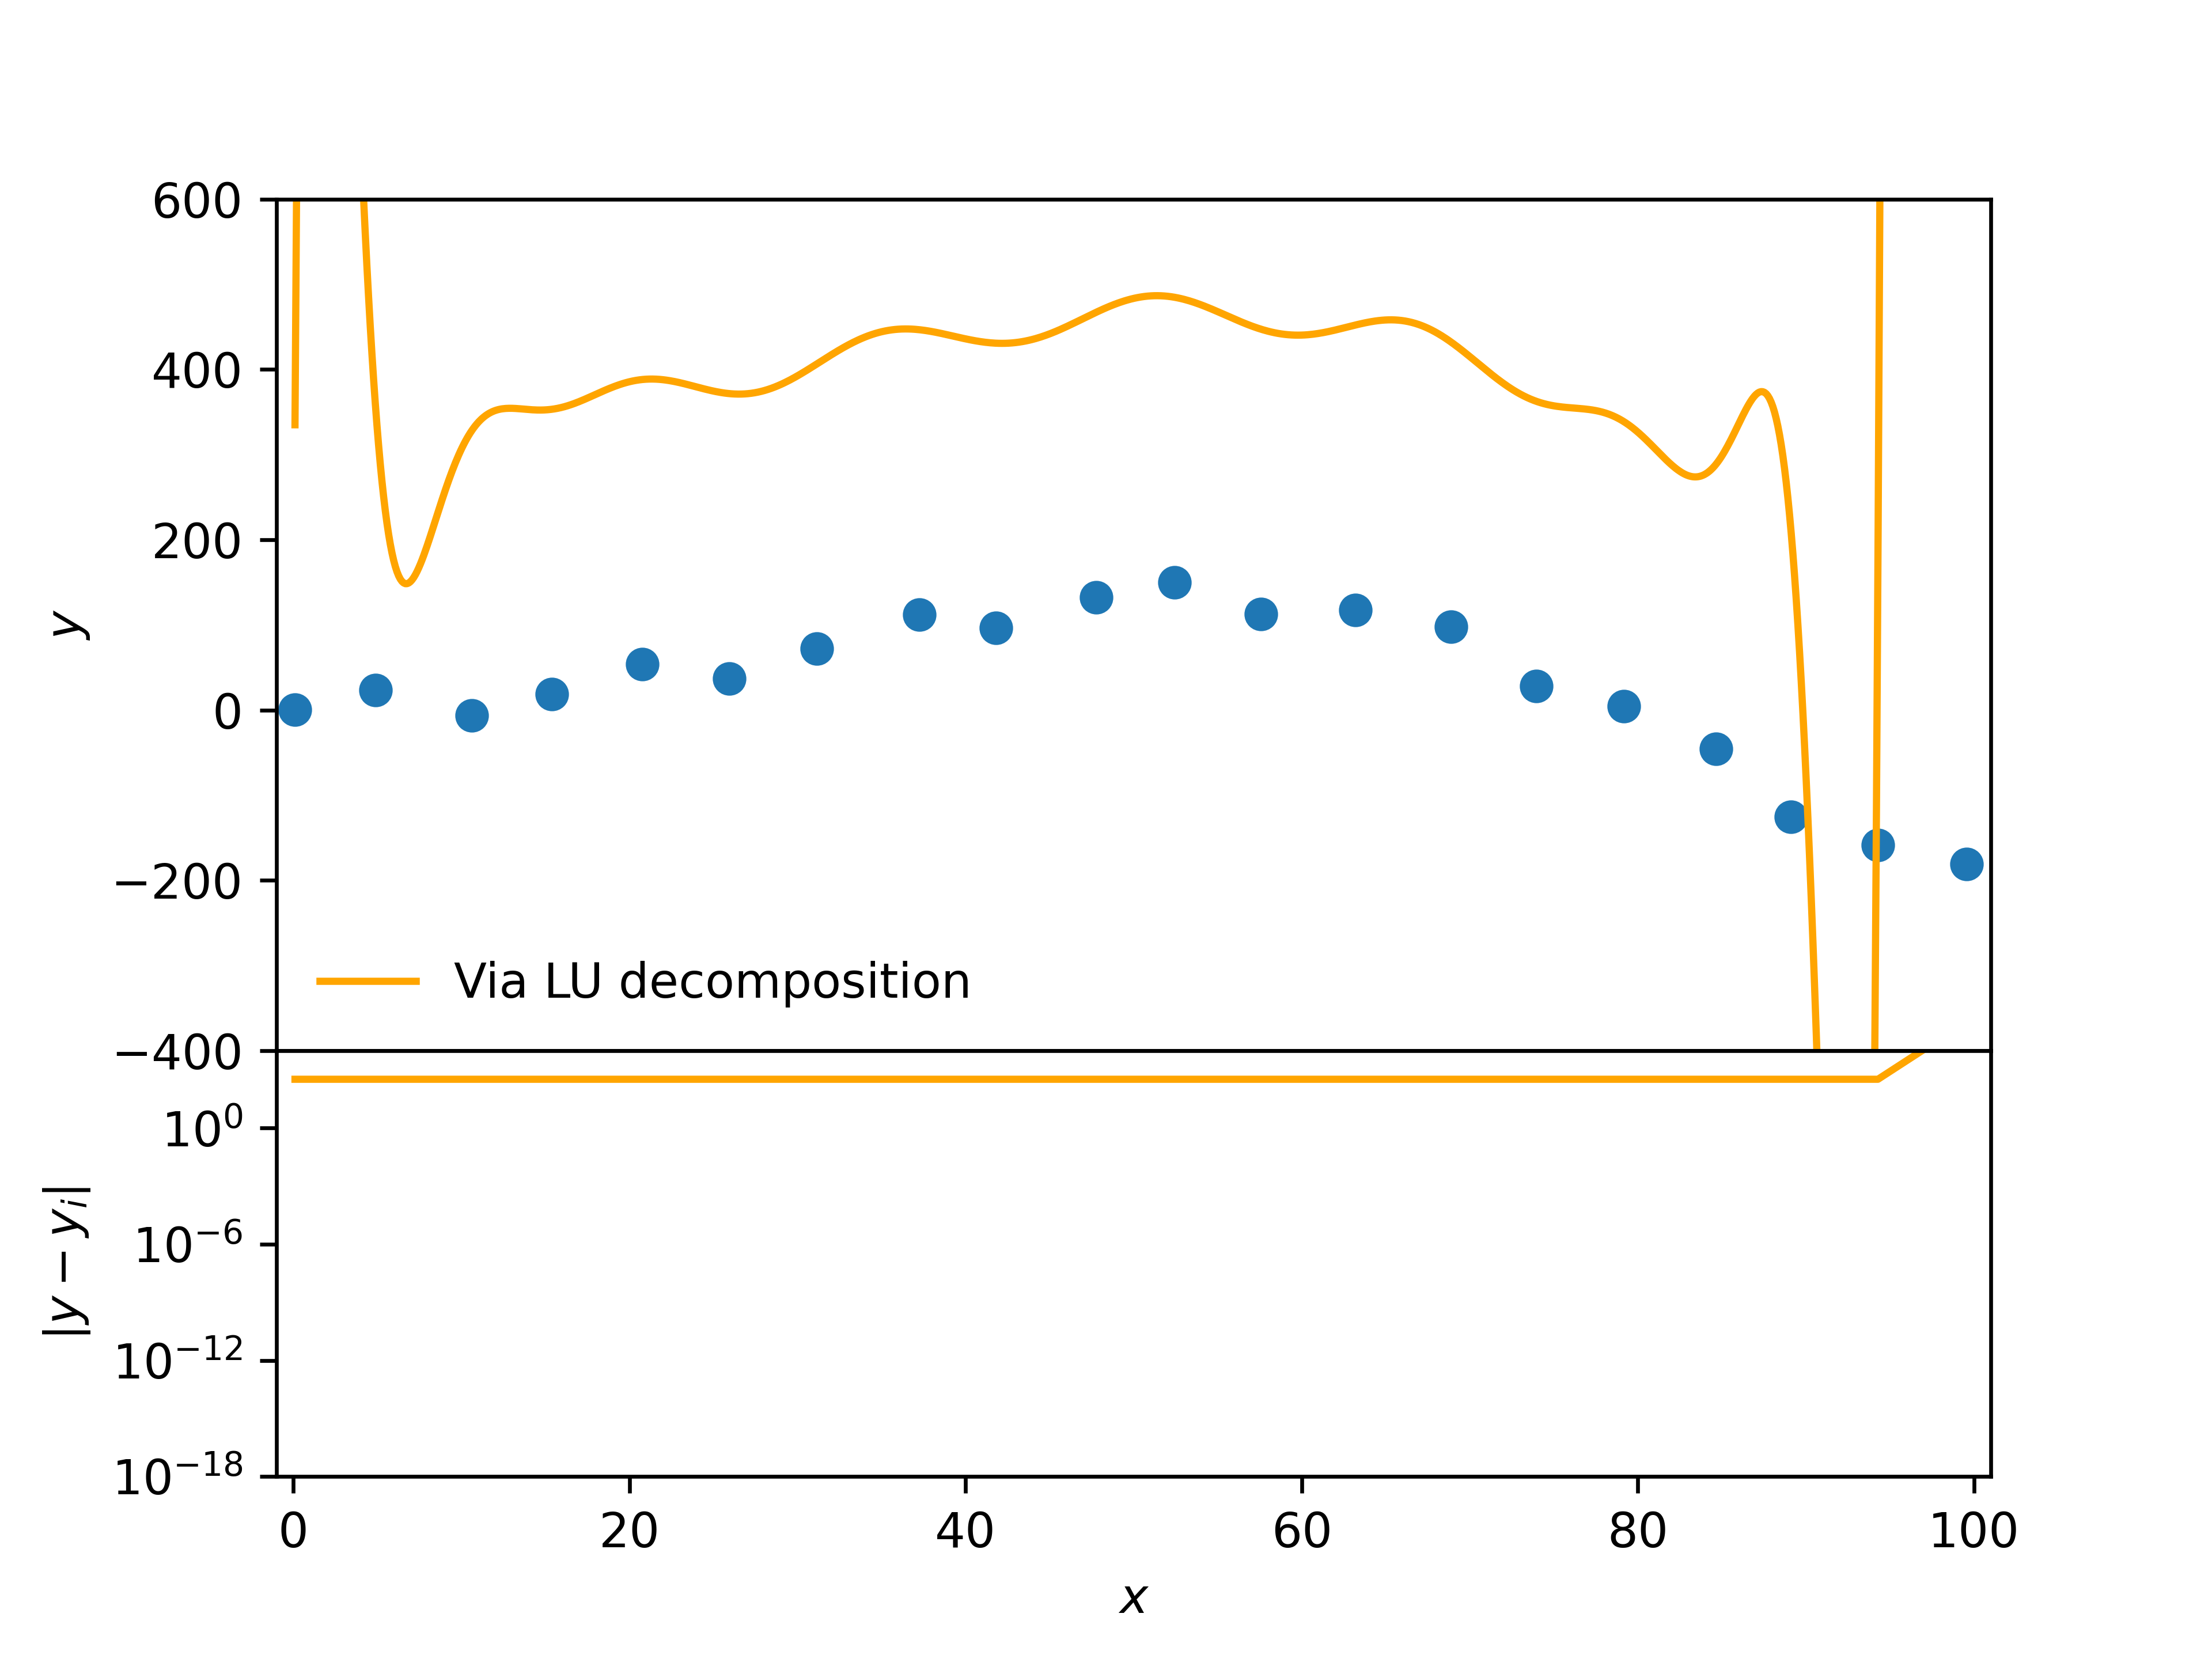
\includegraphics[width=0.9\linewidth]{./my_vandermonde_sol_2a.png}
    \caption{}
    \label{fig:2a}
\end{figure}

\subsection{b}
\lstinputlisting[firstnumber=148, firstline=148, lastline=154]{2_vandermonde_matrix.py}

\begin{figure}[h!]
    \centering
    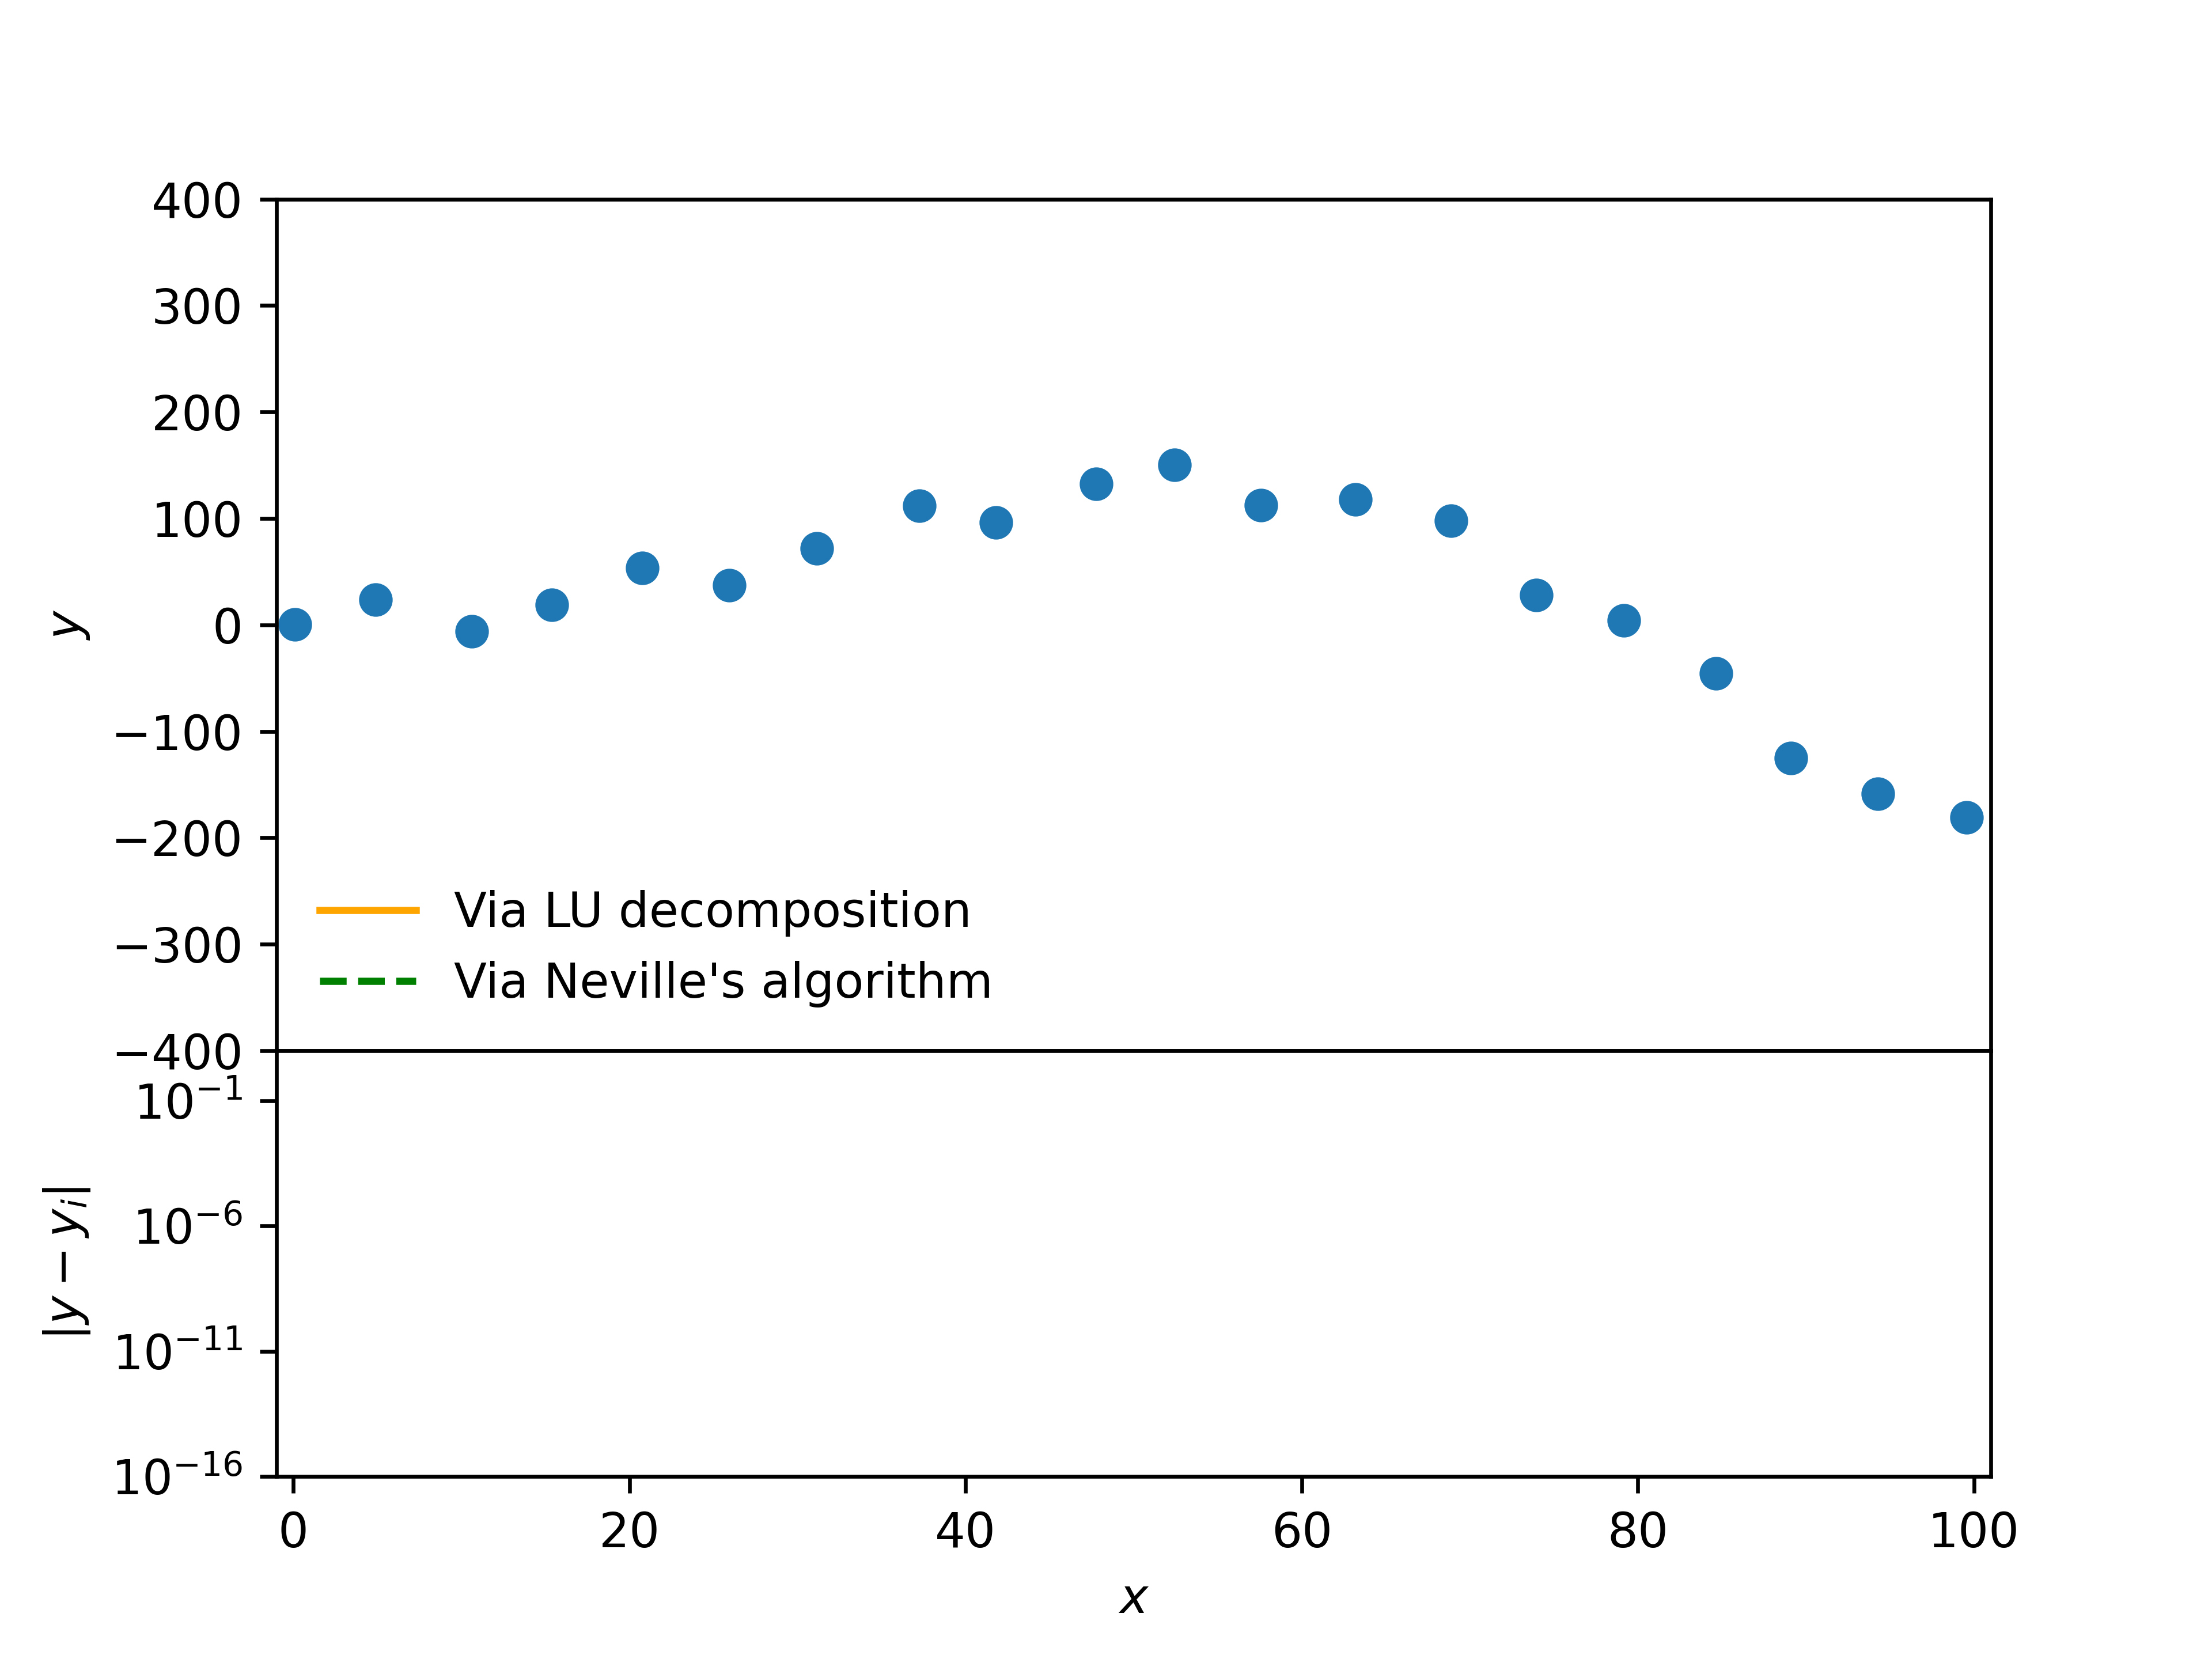
\includegraphics[width=0.9\linewidth]{./my_vandermonde_sol_2b.png}
    \caption{}
    \label{fig:2b}
\end{figure}

\subsection{c}
\lstinputlisting[firstnumber=159, firstline=159, lastline=174]{2_vandermonde_matrix.py}

\begin{figure}[h!]
    \centering
    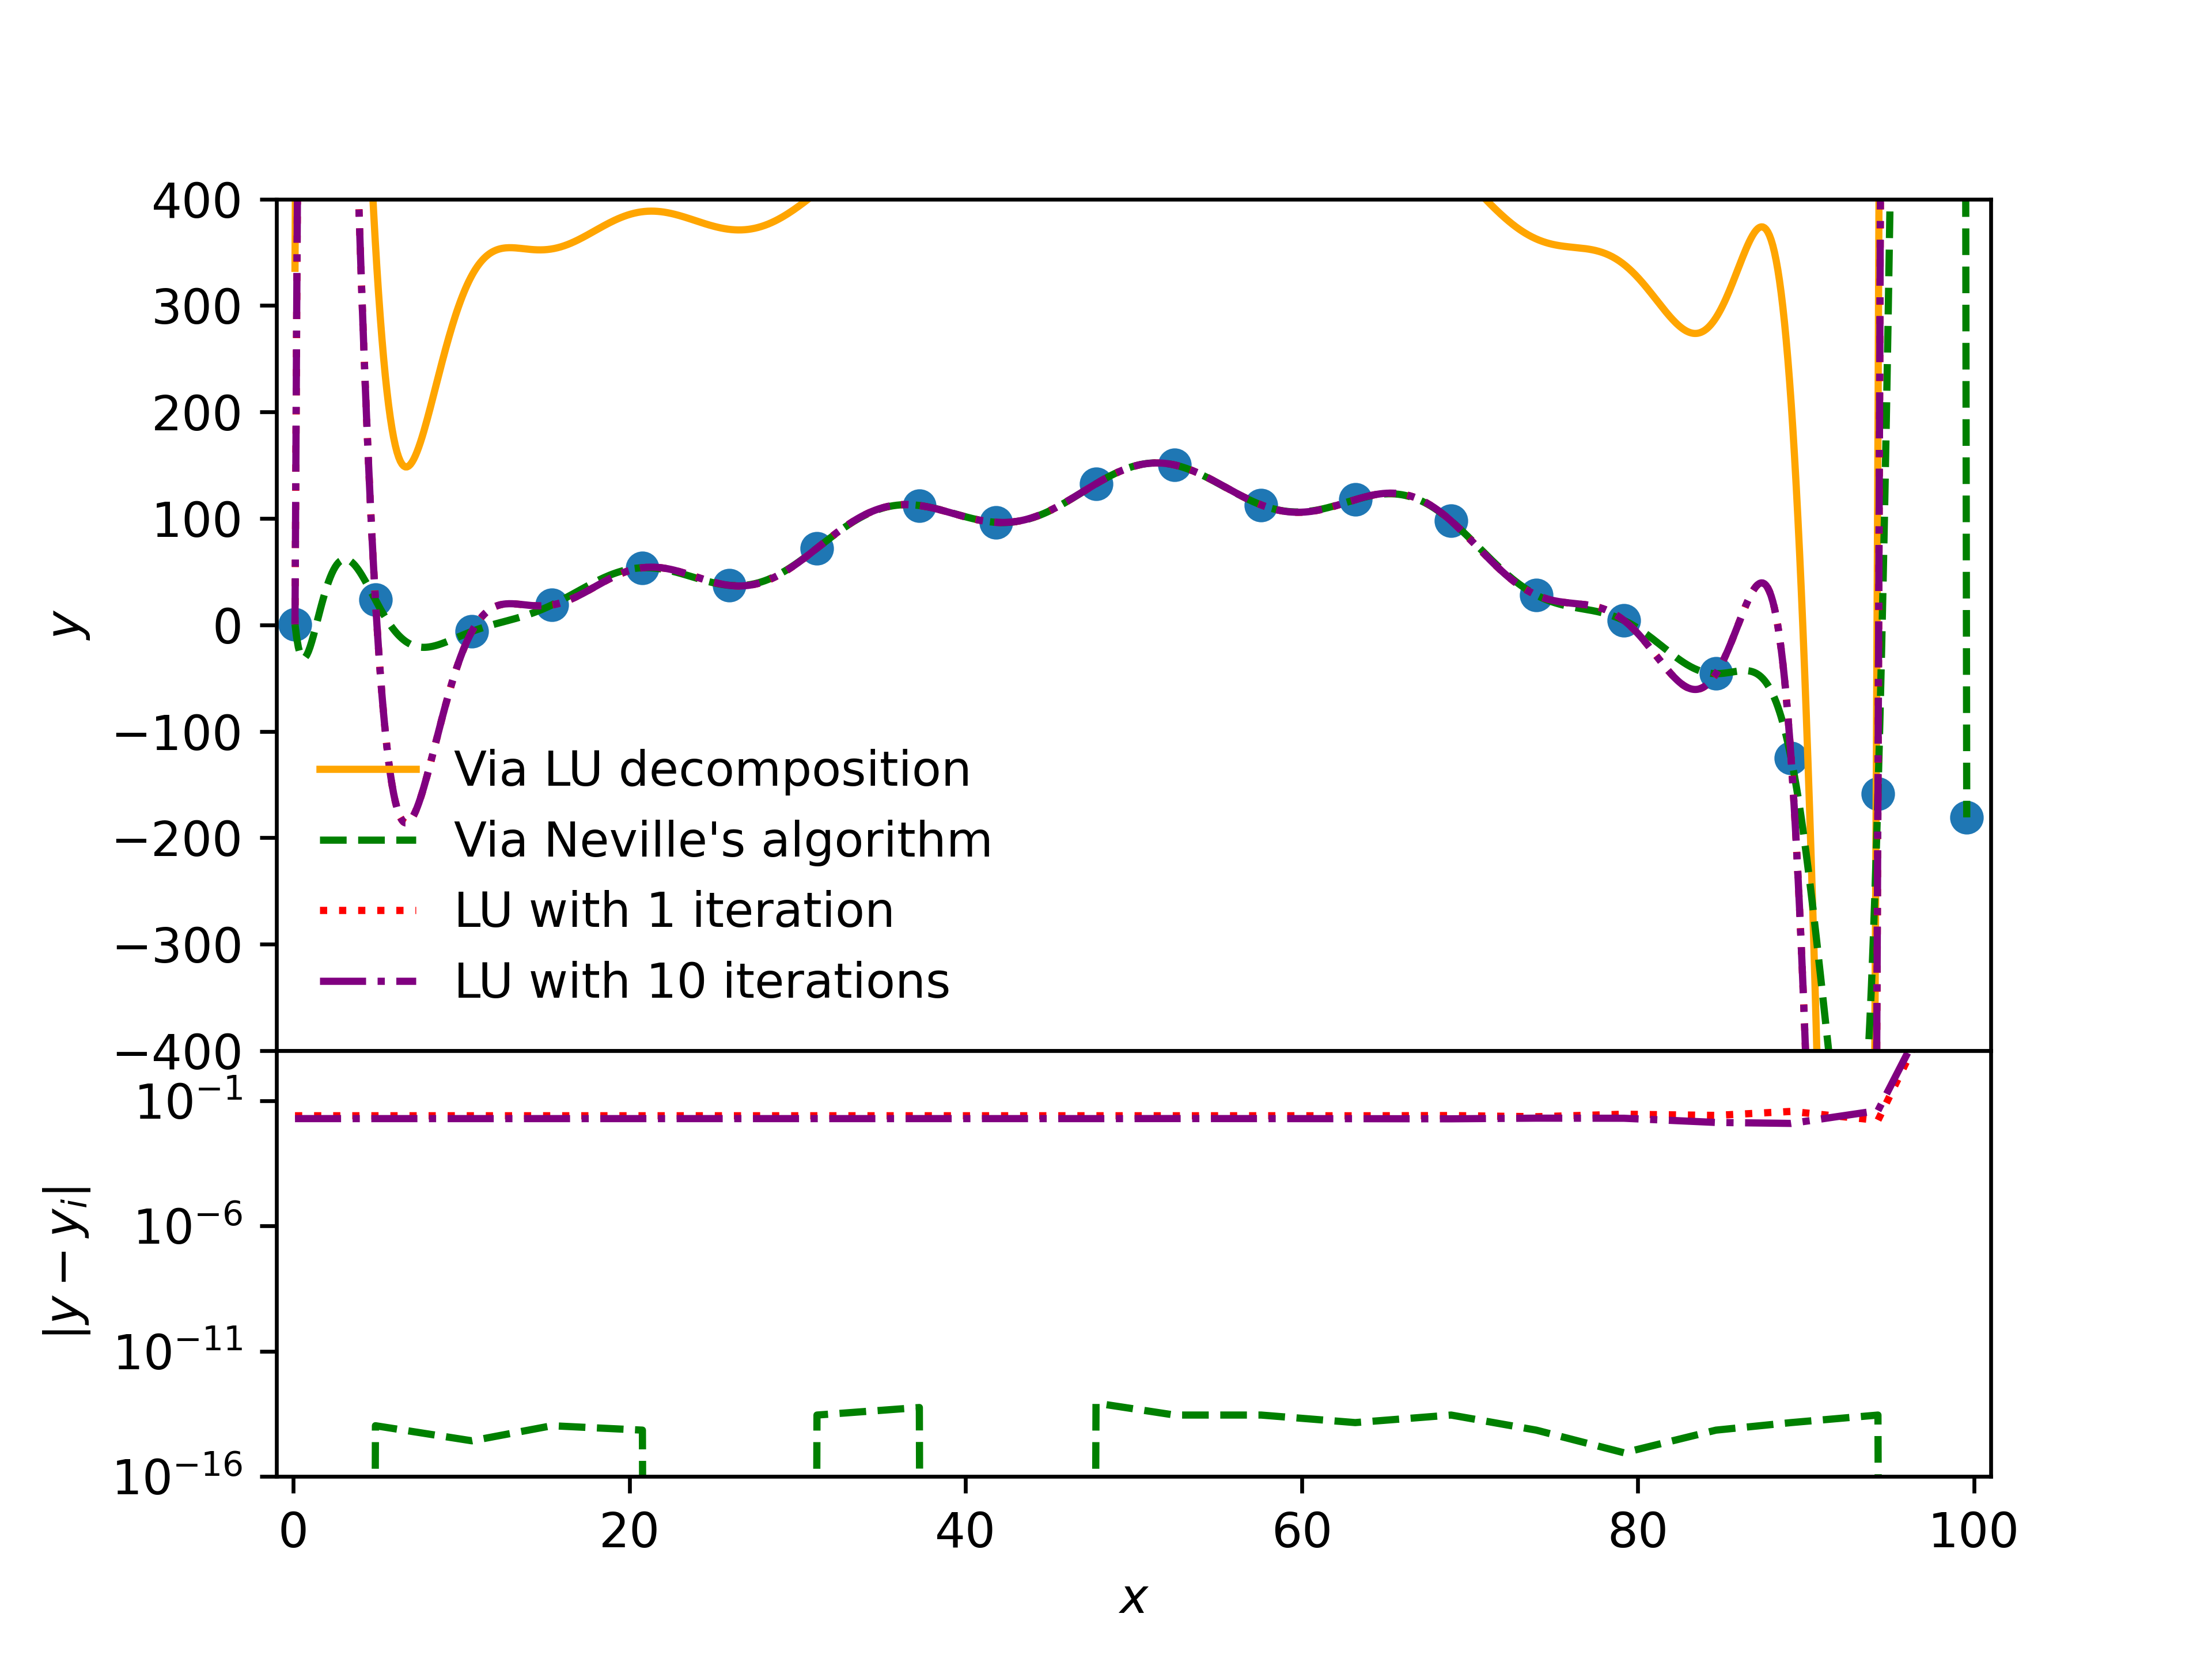
\includegraphics[width=0.9\linewidth]{./my_vandermonde_sol_2c.png}
    \caption{}
    \label{fig:2c}
\end{figure}

\subsection{d}
\lstinputlisting[firstnumber=177, firstline=177, lastline=183]{2_vandermonde_matrix.py}
